\documentclass[11pt]{article}
\usepackage[margin=1in]{geometry}
\usepackage[T1]{fontenc}
\usepackage{lmodern}
\usepackage{microtype}
\usepackage{amsmath,amssymb}
\usepackage{booktabs,array,tabularx}
\usepackage{graphicx}
\usepackage{xcolor}
\usepackage[numbers,sort&compress]{natbib}
\usepackage[hidelinks]{hyperref}
\usepackage{enumitem}
\emergencystretch=2em
\setlist{itemsep=1pt,topsep=3pt,parsep=0pt}
\usepackage{caption}
\captionsetup{font=small,labelfont=bf}

% AUTO-GENERATED by paper/make_numbers.py -- do not edit by hand.
\newcommand{\estHaikuMIXEC}{\ensuremath{-}0.0164}
\newcommand{\loHaikuMIXEC}{\ensuremath{-}0.0205}
\newcommand{\hiHaikuMIXEC}{\ensuremath{-}0.0123}
\newcommand{\holmHaikuMIXEC}{\ensuremath{<}\,0.001}
\newcommand{\estHaikuMIXcStarC}{1.97}
\newcommand{\loHaikuMIXcStarC}{1.69}
\newcommand{\hiHaikuMIXcStarC}{2.25}
\newcommand{\holmHaikuMIXcStarC}{\ensuremath{<}\,0.001}
\newcommand{\estHaikuPUBcStarC}{0.49}
\newcommand{\loHaikuPUBcStarC}{\ensuremath{-}0.01}
\newcommand{\hiHaikuPUBcStarC}{0.99}
\newcommand{\holmHaikuPUBcStarC}{\ensuremath{=}\,0.089}
\newcommand{\estHaikuPUBDC}{0.008}
\newcommand{\loHaikuPUBDC}{\ensuremath{-}0.013}
\newcommand{\hiHaikuPUBDC}{0.030}
\newcommand{\holmHaikuPUBDC}{\ensuremath{=}\,0.776}
\newcommand{\estLunaMIXEC}{\ensuremath{-}0.0165}
\newcommand{\loLunaMIXEC}{\ensuremath{-}0.0214}
\newcommand{\hiLunaMIXEC}{\ensuremath{-}0.0117}
\newcommand{\holmLunaMIXEC}{\ensuremath{<}\,0.001}
\newcommand{\estLunaMIXcStarC}{1.81}
\newcommand{\loLunaMIXcStarC}{1.40}
\newcommand{\hiLunaMIXcStarC}{2.22}
\newcommand{\holmLunaMIXcStarC}{\ensuremath{<}\,0.001}
\newcommand{\estLunaPUBcStarC}{0.65}
\newcommand{\loLunaPUBcStarC}{0.26}
\newcommand{\hiLunaPUBcStarC}{1.05}
\newcommand{\holmLunaPUBcStarC}{\ensuremath{=}\,0.170}
\newcommand{\estLunaPUBDC}{\ensuremath{-}0.005}
\newcommand{\loLunaPUBDC}{\ensuremath{-}0.026}
\newcommand{\hiLunaPUBDC}{0.015}
\newcommand{\holmLunaPUBDC}{\ensuremath{=}\,0.302}
\newcommand{\estSonnetMIXEC}{\ensuremath{-}0.0297}
\newcommand{\loSonnetMIXEC}{\ensuremath{-}0.0430}
\newcommand{\hiSonnetMIXEC}{\ensuremath{-}0.0164}
\newcommand{\holmSonnetMIXEC}{\ensuremath{<}\,0.001}
\newcommand{\estSonnetMIXcStarC}{1.96}
\newcommand{\loSonnetMIXcStarC}{1.67}
\newcommand{\hiSonnetMIXcStarC}{2.25}
\newcommand{\holmSonnetMIXcStarC}{\ensuremath{<}\,0.001}
\newcommand{\estSonnetPUBcStarC}{\ensuremath{-}0.03}
\newcommand{\loSonnetPUBcStarC}{\ensuremath{-}0.89}
\newcommand{\hiSonnetPUBcStarC}{0.83}
\newcommand{\holmSonnetPUBcStarC}{\ensuremath{=}\,0.039}
\newcommand{\estSonnetPUBDC}{\ensuremath{-}0.002}
\newcommand{\loSonnetPUBDC}{\ensuremath{-}0.028}
\newcommand{\hiSonnetPUBDC}{0.024}
\newcommand{\holmSonnetPUBDC}{\ensuremath{=}\,0.441}
\newcommand{\estSolMIXEC}{\ensuremath{-}0.0193}
\newcommand{\loSolMIXEC}{\ensuremath{-}0.0282}
\newcommand{\hiSolMIXEC}{\ensuremath{-}0.0105}
\newcommand{\holmSolMIXEC}{\ensuremath{<}\,0.001}
\newcommand{\estSolMIXcStarC}{3.17}
\newcommand{\loSolMIXcStarC}{2.06}
\newcommand{\hiSolMIXcStarC}{4.28}
\newcommand{\holmSolMIXcStarC}{\ensuremath{<}\,0.001}
\newcommand{\estSolPUBcStarC}{0.50}
\newcommand{\loSolPUBcStarC}{\ensuremath{-}1.08}
\newcommand{\hiSolPUBcStarC}{2.07}
\newcommand{\holmSolPUBcStarC}{\ensuremath{=}\,0.533}
\newcommand{\estSolPUBDC}{\ensuremath{-}0.007}
\newcommand{\loSolPUBDC}{\ensuremath{-}0.020}
\newcommand{\hiSolPUBDC}{0.005}
\newcommand{\holmSolPUBDC}{\ensuremath{=}\,0.259}
\newcommand{\oracleFracHaiku}{0.62}
\newcommand{\oracleFracLoHaiku}{0.47}
\newcommand{\oracleFracHiHaiku}{0.78}
\newcommand{\eOneCommonHaiku}{\ensuremath{-}0.027}
\newcommand{\eOnePubHaiku}{0.000}
\newcommand{\eOnePubLoHaiku}{\ensuremath{-}0.007}
\newcommand{\eOnePubHiHaiku}{0.007}
\newcommand{\cfGainHaiku}{\ensuremath{-}0.0059}
\newcommand{\cfGainLoHaiku}{\ensuremath{-}0.0095}
\newcommand{\cfGainHiHaiku}{\ensuremath{-}0.0022}
\newcommand{\cfGainPubHaiku}{\ensuremath{-}0.0004}
\newcommand{\cfGainPubLoHaiku}{\ensuremath{-}0.0035}
\newcommand{\cfGainPubHiHaiku}{0.0027}
\newcommand{\cDiffHaiku}{1.48}
\newcommand{\cDiffLoHaiku}{0.99}
\newcommand{\cDiffHiHaiku}{2.02}
\newcommand{\oracleFracLuna}{0.63}
\newcommand{\oracleFracLoLuna}{0.49}
\newcommand{\oracleFracHiLuna}{0.76}
\newcommand{\eOneCommonLuna}{\ensuremath{-}0.027}
\newcommand{\eOnePubLuna}{\ensuremath{-}0.003}
\newcommand{\eOnePubLoLuna}{\ensuremath{-}0.009}
\newcommand{\eOnePubHiLuna}{0.004}
\newcommand{\cfGainLuna}{\ensuremath{-}0.0049}
\newcommand{\cfGainLoLuna}{\ensuremath{-}0.0085}
\newcommand{\cfGainHiLuna}{\ensuremath{-}0.0011}
\newcommand{\cfGainPubLuna}{\ensuremath{-}0.0003}
\newcommand{\cfGainPubLoLuna}{\ensuremath{-}0.0024}
\newcommand{\cfGainPubHiLuna}{0.0019}
\newcommand{\cDiffLuna}{1.15}
\newcommand{\cDiffLoLuna}{0.65}
\newcommand{\cDiffHiLuna}{1.67}
\newcommand{\oracleFracSonnet}{0.78}
\newcommand{\oracleFracLoSonnet}{0.53}
\newcommand{\oracleFracHiSonnet}{1.02}
\newcommand{\eOneCommonSonnet}{\ensuremath{-}0.030}
\newcommand{\eOnePubSonnet}{0.006}
\newcommand{\eOnePubLoSonnet}{\ensuremath{-}0.003}
\newcommand{\eOnePubHiSonnet}{0.016}
\newcommand{\cfGainSonnet}{\ensuremath{-}0.0123}
\newcommand{\cfGainLoSonnet}{\ensuremath{-}0.0187}
\newcommand{\cfGainHiSonnet}{\ensuremath{-}0.0065}
\newcommand{\cfGainPubSonnet}{\ensuremath{-}0.0035}
\newcommand{\cfGainPubLoSonnet}{\ensuremath{-}0.0173}
\newcommand{\cfGainPubHiSonnet}{0.0121}
\newcommand{\cDiffSonnet}{1.99}
\newcommand{\cDiffLoSonnet}{0.90}
\newcommand{\cDiffHiSonnet}{3.38}
\newcommand{\oracleFracSol}{0.51}
\newcommand{\oracleFracLoSol}{0.33}
\newcommand{\oracleFracHiSol}{0.68}
\newcommand{\eOneCommonSol}{\ensuremath{-}0.019}
\newcommand{\eOnePubSol}{0.000}
\newcommand{\eOnePubLoSol}{\ensuremath{-}0.008}
\newcommand{\eOnePubHiSol}{0.008}
\newcommand{\cfGainSol}{\ensuremath{-}0.0233}
\newcommand{\cfGainLoSol}{\ensuremath{-}0.0341}
\newcommand{\cfGainHiSol}{\ensuremath{-}0.0125}
\newcommand{\cfGainPubSol}{0.0028}
\newcommand{\cfGainPubLoSol}{\ensuremath{-}0.0013}
\newcommand{\cfGainPubHiSol}{0.0076}
\newcommand{\cDiffSol}{2.67}
\newcommand{\cDiffLoSol}{0.70}
\newcommand{\cDiffHiSol}{4.58}
\newcommand{\baseEqualmeanHaiku}{\ensuremath{-}0.018}
\newcommand{\baseEqualmeanLuna}{\ensuremath{-}0.017}
\newcommand{\baseEqualmeanSonnet}{\ensuremath{-}0.036}
\newcommand{\baseEqualmeanSol}{\ensuremath{-}0.019}
\newcommand{\baseMedianHaiku}{\ensuremath{-}0.014}
\newcommand{\baseMedianLuna}{\ensuremath{-}0.012}
\newcommand{\baseMedianSonnet}{\ensuremath{-}0.030}
\newcommand{\baseMedianSol}{\ensuremath{-}0.013}
\newcommand{\baseUntunedinverHaiku}{\ensuremath{-}0.011}
\newcommand{\baseUntunedinverLuna}{\ensuremath{-}0.009}
\newcommand{\baseUntunedinverSonnet}{\ensuremath{-}0.027}
\newcommand{\baseUntunedinverSol}{\ensuremath{-}0.010}
\newcommand{\baseSameLLMnorecHaiku}{\ensuremath{-}0.016}
\newcommand{\baseSameLLMnorecLuna}{\ensuremath{-}0.017}
\newcommand{\baseSameLLMnorecSonnet}{\ensuremath{-}0.030}
\newcommand{\baseSameLLMnorecSol}{\ensuremath{-}0.019}
\newcommand{\baseTopbyrawscorHaiku}{\ensuremath{-}0.002}
\newcommand{\baseTopbyrawscorLuna}{0.000}
\newcommand{\baseTopbyrawscorSonnet}{\ensuremath{-}0.004}
\newcommand{\baseTopbyrawscorSol}{\ensuremath{+}0.013}
\newcommand{\baseCVperfweightHaiku}{\ensuremath{+}0.004}
\newcommand{\baseCVperfweightLuna}{\ensuremath{+}0.006}
\newcommand{\baseCVperfweightSonnet}{\ensuremath{+}0.003}
\newcommand{\baseCVperfweightSol}{\ensuremath{+}0.020}
\newcommand{\baseGrouporaclesHaiku}{\ensuremath{+}0.008}
\newcommand{\baseGrouporaclesLuna}{\ensuremath{+}0.010}
\newcommand{\baseGrouporaclesSonnet}{\ensuremath{+}0.002}
\newcommand{\baseGrouporaclesSol}{\ensuremath{+}0.019}
\newcommand{\pubBrierMeanHaiku}{0.1689}
\newcommand{\pubBrierWHaiku}{0.1695}
\newcommand{\pubBrierMeanLuna}{0.1689}
\newcommand{\pubBrierWLuna}{0.1695}
\newcommand{\inflRaw}{\ensuremath{+}0.0179}
\newcommand{\inflRawLo}{0.0097}
\newcommand{\inflRawHi}{0.0260}
\newcommand{\inflPeer}{\ensuremath{-}0.0056}
\newcommand{\inflPeerLo}{\ensuremath{-}0.0118}
\newcommand{\inflPeerHi}{0.0007}
\newcommand{\inflFe}{\ensuremath{-}0.0060}
\newcommand{\inflFeLo}{\ensuremath{-}0.0121}
\newcommand{\inflFeHi}{0.0001}
\newcommand{\inflRawAbs}{0.018}
\newcommand{\inflN}{4{,}283}
\newcommand{\inflTercA}{\ensuremath{+}0.048}
\newcommand{\inflTercB}{\ensuremath{+}0.031}
\newcommand{\inflTercC}{\ensuremath{-}0.023}
\newcommand{\normRaw}{\ensuremath{+}0.005}
\newcommand{\normRawLo}{\ensuremath{-}0.023}
\newcommand{\normRawHi}{0.033}
\newcommand{\normSeedsMean}{\ensuremath{+}0.019}
\newcommand{\normSeedsMin}{\ensuremath{-}0.004}
\newcommand{\normSeedsMax}{\ensuremath{+}0.043}
\newcommand{\normSeedsN}{20}
\newcommand{\nonceShiftHaikuCtwo}{\ensuremath{-}0.0124}
\newcommand{\nonceShiftHaikuCthree}{\ensuremath{-}0.0005}
\newcommand{\nonceShiftLunaCtwo}{\ensuremath{+}0.0011}
\newcommand{\nonceShiftLunaCthree}{\ensuremath{-}0.0032}
\newcommand{\nonceShiftSonnetCtwo}{\ensuremath{+}0.0038}
\newcommand{\nonceShiftSolCtwo}{\ensuremath{+}0.0005}
\newcommand{\nonceHaikuN}{373}
\newcommand{\nonceHaikuD}{\ensuremath{-}0.029}
\newcommand{\placeboHaikuDtwo}{\ensuremath{-}0.034}
\newcommand{\probeHaiku}{0.146}
\newcommand{\probeLuna}{0.133}
\newcommand{\probeSonnet}{0.120}
\newcommand{\probeSol}{0.134}
\newcommand{\probeCrowdLo}{0.140}
\newcommand{\probeCrowdHi}{0.144}
\newcommand{\slopeHaikuMix}{2.3}
\newcommand{\slopeHaikuPub}{2.6}
\newcommand{\slopeLunaMix}{2.7}
\newcommand{\slopeLunaPub}{3.3}
\newcommand{\slopeSonnetMix}{2.5}
\newcommand{\slopeSonnetPub}{2.7}
\newcommand{\slopeSolMix}{2.0}
\newcommand{\slopeSolPub}{2.2}
\newcommand{\sonnetPubHolmFrozen}{0.039}
\newcommand{\sonnetPubHolmExact}{0.060}
\newcommand{\sonnetPubHolmCons}{0.133}
\newcommand{\noiseCorrPubHaikuA}{0.47}
\newcommand{\noiseCorrPubHaikuB}{0.71}
\newcommand{\noiseCorrPubLunaA}{0.69}
\newcommand{\noiseCorrPubLunaB}{0.72}
\newcommand{\mdeMin}{0.016}
\newcommand{\mdeMax}{0.033}
\newcommand{\betaBaseMin}{0.42}
\newcommand{\betaBaseMax}{0.65}
\newcommand{\betaStarEff}{1.28}
\newcommand{\betaStarStrong}{1.71}
\newcommand{\oracleFracCthreeHaiku}{0.23}
\newcommand{\oracleFracConeHaiku}{\ensuremath{-}0.16}
\newcommand{\oracleFracCthreeLuna}{0.45}
\newcommand{\oracleFracConeLuna}{0.59}
\newcommand{\oracleFracCthreeSonnet}{0.41}
\newcommand{\oracleFracConeSonnet}{0.13}
\newcommand{\oracleFracCthreeSol}{0.26}
\newcommand{\oracleFracConeSol}{0.53}
\newcommand{\pooledWHaiku}{\ensuremath{+}0.0026}
\newcommand{\pooledWLoHaiku}{0.0002}
\newcommand{\pooledWHiHaiku}{0.0052}
\newcommand{\pooledWLuna}{\ensuremath{+}0.0043}
\newcommand{\pooledWLoLuna}{0.0020}
\newcommand{\pooledWHiLuna}{0.0065}
\newcommand{\pooledWSonnet}{\ensuremath{-}0.0045}
\newcommand{\pooledWLoSonnet}{\ensuremath{-}0.0096}
\newcommand{\pooledWHiSonnet}{0.0010}
\newcommand{\pooledWSol}{\ensuremath{+}0.0124}
\newcommand{\pooledWLoSol}{0.0085}
\newcommand{\pooledWHiSol}{0.0161}
\newcommand{\pooledWBrier}{0.1156}
\newcommand{\typedWBrier}{0.1130}
\newcommand{\statedSuperMin}{0.53}
\newcommand{\statedSuperMax}{0.65}
\newcommand{\revealedShareMin}{0.30}
\newcommand{\revealedShareMax}{0.66}
\newcommand{\pwGapMax}{0.032}
\newcommand{\pwMinusLlmMin}{\ensuremath{-}0.0007}
\newcommand{\pwMinusLlmMax}{\ensuremath{+}0.0011}
\newcommand{\pooledWAllHaiku}{\ensuremath{-}0.0006}
\newcommand{\pooledWAllLoHaiku}{\ensuremath{-}0.0033}
\newcommand{\pooledWAllHiHaiku}{0.0020}
\newcommand{\pooledWAllLuna}{\ensuremath{+}0.0004}
\newcommand{\pooledWAllLoLuna}{\ensuremath{-}0.0017}
\newcommand{\pooledWAllHiLuna}{0.0025}
\newcommand{\pooledWAllSonnet}{\ensuremath{-}0.0080}
\newcommand{\pooledWAllLoSonnet}{\ensuremath{-}0.0133}
\newcommand{\pooledWAllHiSonnet}{\ensuremath{-}0.0026}
\newcommand{\pooledWAllSol}{\ensuremath{+}0.0034}
\newcommand{\pooledWAllLoSol}{\ensuremath{-}0.0017}
\newcommand{\pooledWAllHiSol}{0.0079}
\newcommand{\pooledWMaskedHaiku}{\ensuremath{+}0.0014}
\newcommand{\statedShiftMin}{0.30}
\newcommand{\statedShiftMax}{0.54}
\newcommand{\haikuCommonW}{\ensuremath{+}0.011}
\newcommand{\haikuCommonWse}{0.004}
\newcommand{\nonceTokFarm}{318}
\newcommand{\nonceTokCtl}{122}
\newcommand{\nonceTokFarmAll}{337}
\newcommand{\nonceTokCtlAll}{137}
\newcommand{\swapMin}{\ensuremath{-}1.05}
\newcommand{\swapMax}{\ensuremath{-}0.15}
\newcommand{\swapHaiku}{\ensuremath{-}0.70}
\newcommand{\swapSeHaiku}{0.18}
\newcommand{\swapLuna}{\ensuremath{-}1.05}
\newcommand{\swapSeLuna}{0.17}
\newcommand{\pubWHaiku}{\ensuremath{-}0.0035}
\newcommand{\pubWLoHaiku}{\ensuremath{-}0.0084}
\newcommand{\pubWHiHaiku}{0.0013}
\newcommand{\pubWLuna}{\ensuremath{-}0.0032}
\newcommand{\pubWLoLuna}{\ensuremath{-}0.0072}
\newcommand{\pubWHiLuna}{0.0009}
\newcommand{\pubWSonnet}{\ensuremath{-}0.0113}
\newcommand{\pubWLoSonnet}{\ensuremath{-}0.0199}
\newcommand{\pubWHiSonnet}{\ensuremath{-}0.0038}
\newcommand{\pubWSol}{\ensuremath{-}0.0054}
\newcommand{\pubWLoSol}{\ensuremath{-}0.0131}
\newcommand{\pubWHiSol}{0.0014}
\newcommand{\eOneAbsHaiku}{0.016}
\newcommand{\eOneAbsLuna}{0.017}
\newcommand{\eOneCommonAbsMin}{0.019}
\newcommand{\eOneCommonAbsMax}{0.030}

\newcommand{\cstar}{c^{*}}

\title{The Ledger Test: Can Reliability Scores Improve---or Corrupt---AI Forecast Aggregation?}
\author{[Author names withheld for review]\\\small Apart Research AI $\times$ Epistemics Sprint, Trust Infrastructure track}
\date{November 2026}

\begin{document}
\maketitle

\begin{abstract}
\noindent
LLMs are increasingly asked to combine other people's judgements, and reliability metadata such as track records and
accuracy scores is the obvious thing to show them. We test whether showing such metadata to an LLM aggregator helps,
how much the model relies on it, and whether the metadata can be gamed. We use real individual forecasts from
ForecastBench's 2024-07-21 human round (162 resolved binary questions) and build 972 frozen five-person panels, either
mixed (MIX: two superforecasters, three public forecasters) or all-public (PUB). Four LLMs (two efficient, two
strong) see the same forecasts under four presentations of the forecasters' records, plus paired interventions that
swap or ``farm'' a record while the forecasts stay fixed. The confirmatory estimands and tests were pre-specified
and frozen before data collection; analyses added afterwards are labelled post hoc. In MIX panels, one raw accuracy
number per forecaster lowers the LLM's Brier score for all four models (Holm-adjusted $p<0.001$): by
\eOneAbsHaiku--\eOneAbsLuna{} for the two efficient models on all 486 panels, and by
\eOneCommonAbsMin--\eOneCommonAbsMax{} on the 108 panels that all four models share. This captures roughly half to
three-quarters of the gain of knowing who the experts are. But no model beats a simple performance-weighted average
tuned by cross-validation for that panel type, and in PUB panels records give no measurable benefit. In MIX every
model moves too little: rescaling its record-induced shift by a factor fitted on other questions improves held-out
accuracy. However, the models respond to scores in the same way whether or not experts are present. Padding a record
with easy, confident forecasts improves its displayed raw mean Brier by \inflRawAbs{} on average (95\% CI
[\inflRawLo, \inflRawHi]), and peer-relative or difficulty-adjusted scores remove this. The inflation is modest,
reverses for the weakest forecasters, and did not make the score less predictive in these data. Our test of whether
LLMs discount farmed records is not identified: a cache-busting line that we added to the control prompts changed one
model's behaviour. We report this flaw in full. For trust infrastructure, reliability scores help AI aggregators when
real skill differences exist, transparent statistical weighting is a strong default when the right rule for the
regime is known, and peer-relative scoring removes the one form of record padding we could measure.
\end{abstract}

\section{Introduction}
Forecast aggregation is an epistemic primitive: decision-makers rarely consult a single forecaster, and the
choice of whom to trust is often made with the help of track records. As LLM assistants are deployed to
summarise and combine expert judgement, the reliability metadata attached to those judgements (leaderboards, Brier
scores, ``verified forecaster'' badges) becomes an input to the model. This creates two questions that matter for
trust infrastructure. First, \emph{utility}: does the metadata actually improve the AI's aggregate, and does the model
weight it appropriately? Second, \emph{integrity}: can a forecaster game the metadata (for example, by
forecasting confidently on easy questions to pad their record), and does the choice of score make such gaming
harmless?

The classical literature shows that the simple average is hard to beat \citep{clemen1989}, that performance-based
selection or contribution weighting can help when skill differences are real \citep{budescu2015,mannes2014}, and that
leaderboards create strategic incentives even under proper scoring rules \citep{witkowski2018}. Recent work shows that
LLMs recognise reliability cues without always using them \citep{zhang2026}, and that they weight source popularity more
than reliability \citep{ashkinaze2026}. What is missing is a test with \emph{real} human track records, an LLM producing a
\emph{probability} scored against \emph{real outcomes}, and \emph{paired interventions} on the metadata alone.

\paragraph{Contributions.}
\begin{enumerate}
\item A pre-specified benchmark design (frozen in a commit before the main run), the \emph{Ledger Test}, built on ForecastBench human forecasts
  \citep{karger2025}. It holds the forecasts fixed and varies only the reliability block: no records, itemised records,
  a raw mean Brier, or a peer-relative score. It adds record-swap and record-farming interventions.
\item Evidence from four LLMs that raw scores improve aggregation when experts are present, but by less than a transparent
  statistical rule tuned for the panel type, and not at all in all-public panels (RQ1).
\item A reliance estimand, $\cstar$, that needs no statistical benchmark. It shows MIX under-reaction that survives cross-fitting, together with
  evidence that the models' policy is regime-blind (RQ2).
\item A data-level measurement of record farming and of the protection offered by peer-relative and difficulty-adjusted
  scores (RQ3a). We also give a candid account of why our LLM-level farming test is not identified (RQ3b), with
  design lessons for future studies.
\end{enumerate}
Code, frozen configurations, all 19,876 raw model responses, and every script that generates a number in this paper
are in the project repository (link in the submission form). Each number in the text is generated from a result file and traced in a claims ledger
(Appendix~\ref{app:repro}).

\section{Related work}
\textbf{Aggregation and reliability weighting.} Equal weighting is a robust default \citep{clemen1989}. Extremising
the mean log-odds improves crowd forecasts \citep{satopaa2014}. Selecting a few top judges can beat averaging all
of them \citep{mannes2014}, and weighting by performance \emph{relative to peers} identifies expertise better than absolute
accuracy \citep{budescu2015}. Our peer-relative condition (C3) is in the spirit of this approach. We score with the Brier
score \citep{brier1950}.
\textbf{LLMs and source reliability.} \citet{zhang2026} show, in synthetic scenarios, that LLMs can recognise
epistemic cues without being influenced by them, and that exchanging source histories can reverse choices. Our
record-swap check builds directly on that precedent. \citet{ashkinaze2026} find that models rely on source popularity
about twice as much as on reliability. Neither study uses real forecaster records, continuous probabilities, or
downstream proper-scoring loss.
\textbf{LLM forecasting and crowds.} ForecastBench \citep{karger2025} supplies our data; its later leaderboard
methodology motivates difficulty-adjusted scoring. \citet{schoenegger2024} and \citet{douven2026} study crowds \emph{of} LLM forecasters
combined statistically; we study an LLM \emph{as} the aggregator of human forecasts.
\textbf{Gaming.} \citet{witkowski2018} show that winner-take-all leaderboards make proper scoring rules
non-incentive-compatible through the reported probability. We study a different lever: which questions enter a record.
\textbf{Novelty.} To our knowledge (non-exhaustive search, November 2026), no prior work combines real individual human
records, an LLM aggregator scored by a proper rule, paired metadata-only interventions, and a raw-versus-adjusted score
comparison measured in downstream loss. Each element has a precedent; the combination is our contribution.

\section{Methods}
\subsection{Data and panels}
We use the ForecastBench human round of 2024-07-21 (repository commit \texttt{203a0d1}). After joining on resolutions,
162 binary question ids are resolved and scored. A median of 59 forecasters answered each question. Each panel has five
members labelled A--E in a seeded random order, and the group (public or super) is never shown. \textbf{MIX} panels
contain 3 public forecasters and 2 superforecasters; \textbf{PUB} panels contain 5 public forecasters. We draw 3 panels
per type per question, giving 972 frozen panels. The target question is shown \emph{without its text}, as a random
two-letter category code and a horizon bucket, to limit pretraining knowledge. A text-only probe shows that,
given the question text, the models are about as accurate as the human crowd (Brier \probeSonnet--\probeHaiku{} against
\probeCrowdLo--\probeCrowdHi; Appendix~\ref{app:extra}). Pretraining knowledge is therefore plausible, and the main
prompts rely on withholding the text.

\subsection{Conditions and interventions}
Each member's record shows $k=8$ other resolved questions from the same round, drawn uniformly. The target is always
excluded (leave-one-out). Only the reliability block varies across conditions:
\textbf{C0}, no records;
\textbf{C1}, itemised (category, horizon, forecast and outcome for each of the 8 items);
\textbf{C2}, the raw mean Brier on those 8 items (3 decimals, with ``always 50\% scores 0.250'' as a reference);
\textbf{C3}, a peer-relative Brier (the member's Brier minus the mean of all other forecasters on the same items).
The system prompt asks for the probability that minimises expected Brier score. The model returns JSON with a
probability and a non-negative weight for each member.
\textbf{Swap}: the records of the best- and worst-scored members are exchanged (manipulation check).
\textbf{Farming} (PUB only): an \emph{attacker} is a public member with at least 8 ``confident'' items
($|p-0.5|\ge 0.4$). The farmed record shows 8 of these. A \emph{score-matched control} record is a uniform draw whose
mean raw Brier matches the farmed one within 0.01. Further arms are a test--retest of C2 and the text-only probe.

\subsection{Models and runs}
The efficient tier comprises Claude Haiku 5.5 (\textbf{Haiku}) and GPT-6 Luna (\textbf{Luna}), run on all 486
panels per type. The strong tier comprises Claude Sonnet 5.5 (\textbf{Sonnet}) and GPT-6.1 Sol (\textbf{Sol}), run on a
seeded nested subset of 108 questions at draw 0 for budget reasons. All models were called through OpenRouter with
reasoning effort ``low'' and at most 2,000 output tokens. Sonnet emits no reasoning tokens at this setting. The run
produced 19,876 responses with 0 parse failures, at a cost of \$11.22. Cross-model comparisons use only the
common 108-question draw-0 sample.

\subsection{Estimands and inference}
The confirmatory estimands, samples and tests were frozen in a design document and configuration before the main run. A pilot of
16 questions informed the design; results excluding those 16 questions are reported as a pre-declared sensitivity.
\begin{itemize}
\item \textbf{E1 (RQ1):} $\Delta$Brier $=$ Brier(C2) $-$ Brier(C0) on MIX panels. The descriptive \emph{oracle
  fraction} is $[\text{Brier(C0)}-\text{Brier(C2)}]/[\text{Brier(mean)}-\text{Brier(oracle)}]$, where the oracle is the
  mean of the two superforecasters.
\item \textbf{E2 (RQ2):} with $L$ the LLM's probability and $\Delta L = L_{C2}-L_{C0}$,
  $\cstar = \arg\min_c \sum (L_{C0} + c\,\Delta L - y)^2$, tested against $H_0{:}\ \cstar=1$ separately for MIX and PUB.
  $\cstar>1$ means the model should have moved \emph{further} in the direction it moved. This estimand needs no
  statistical benchmark.
\item \textbf{E3a (RQ3a, no LLM):} the farming inflation of the displayed score, (control $-$ farmed), for raw, peer and
  fixed-effect (difficulty-adjusted) scores, over all \inflN{} eligible attacker--target pairs.
\item \textbf{E3b (RQ3b):} the farming discount
  $D=\sum (L_\text{farm}-L_\text{ctl})\,\mathrm{sign}(g)/\sum|g|$ in C1, where $g$ is the attacker's distance from the
  other members' mean (one-sided, $D<0$).
\end{itemize}
The confirmatory family per model is \{E1, E2-MIX, E2-PUB, E3b\}, with Holm correction \citep{holm1979}. Standard errors
are two-way cluster-robust (question $\times$ forecaster; \citep{cameron2011}), with question-cluster bootstrap CIs
(2,000 replicates) alongside. Statistical comparators include the equal mean, the median, the logit mean, top-2 by score,
an untuned inverse-Brier weighting, and a performance-weighted mean $W$, whose two hyperparameters are tuned on outcomes by 5-fold
cross-validation over questions, separately for MIX and PUB. $W$ therefore knows the panel type; the LLM is not told it.

\section{Results}
Table~\ref{tab:conf} gives the confirmatory family. Every confirmatory estimate was reproduced by independent code
(Appendix~\ref{app:repro}). The cross-fitted, noise-corrected, regime-blind and MIX$-$PUB analyses in \S\ref{sec:rq2},
the heterogeneity, normative and nonce analyses in \S\ref{sec:rq3}, and \S\ref{sec:expl} are post hoc.

\begin{table}[t]
\centering\small
\caption{Confirmatory family, primary sample: estimate, 95\% CI and Holm-adjusted $p$ (4 tests per model). $^\dagger$Depends on the SE convention; not interpreted (\S\ref{sec:rq2}).
Haiku and Luna: 486 panels per type; Sonnet and Sol: 108. E3b is \emph{not identified} (\S\ref{sec:rq3}).}
\label{tab:conf}
\begin{tabular}{@{}l>{\raggedright}p{3.1cm}>{\raggedright}p{2.6cm}>{\raggedright}p{2.6cm}>{\raggedright\arraybackslash}p{3.0cm}@{}}
\toprule
Model & E1: MIX $\Delta$Brier & E2: $\cstar$ MIX & E2: $\cstar$ PUB & E3b: $D_{C1}$ \\
\midrule
Haiku & \ensuremath{-}0.0164 \newline [\ensuremath{-}0.0205, \ensuremath{-}0.0123] \newline \textit{p}\,\ensuremath{<}\,0.001 & 1.97 \newline [1.69, 2.25] \newline \textit{p}\,\ensuremath{<}\,0.001 & 0.49 \newline [\ensuremath{-}0.01, 0.99] \newline \textit{p}\,\ensuremath{=}\,0.089 & 0.008 \newline [\ensuremath{-}0.013, 0.030] \newline \textit{p}\,\ensuremath{=}\,0.776 \\
Luna & \ensuremath{-}0.0165 \newline [\ensuremath{-}0.0214, \ensuremath{-}0.0117] \newline \textit{p}\,\ensuremath{<}\,0.001 & 1.81 \newline [1.40, 2.22] \newline \textit{p}\,\ensuremath{<}\,0.001 & 0.65 \newline [0.26, 1.05] \newline \textit{p}\,\ensuremath{=}\,0.170 & \ensuremath{-}0.005 \newline [\ensuremath{-}0.026, 0.015] \newline \textit{p}\,\ensuremath{=}\,0.302 \\
Sonnet & \ensuremath{-}0.0297 \newline [\ensuremath{-}0.0430, \ensuremath{-}0.0164] \newline \textit{p}\,\ensuremath{<}\,0.001 & 1.96 \newline [1.67, 2.25] \newline \textit{p}\,\ensuremath{<}\,0.001 & \ensuremath{-}0.03 \newline [\ensuremath{-}0.89, 0.83] \newline \textit{p}\,\ensuremath{=}\,0.039$^\dagger$ & \ensuremath{-}0.002 \newline [\ensuremath{-}0.028, 0.024] \newline \textit{p}\,\ensuremath{=}\,0.441 \\
Sol & \ensuremath{-}0.0193 \newline [\ensuremath{-}0.0282, \ensuremath{-}0.0105] \newline \textit{p}\,\ensuremath{<}\,0.001 & 3.17 \newline [2.06, 4.28] \newline \textit{p}\,\ensuremath{<}\,0.001 & 0.50 \newline [\ensuremath{-}1.08, 2.07] \newline \textit{p}\,\ensuremath{=}\,0.533 & \ensuremath{-}0.007 \newline [\ensuremath{-}0.020, 0.005] \newline \textit{p}\,\ensuremath{=}\,0.259 \\
\bottomrule

\end{tabular}
\end{table}

\begin{figure}[t]
\centering
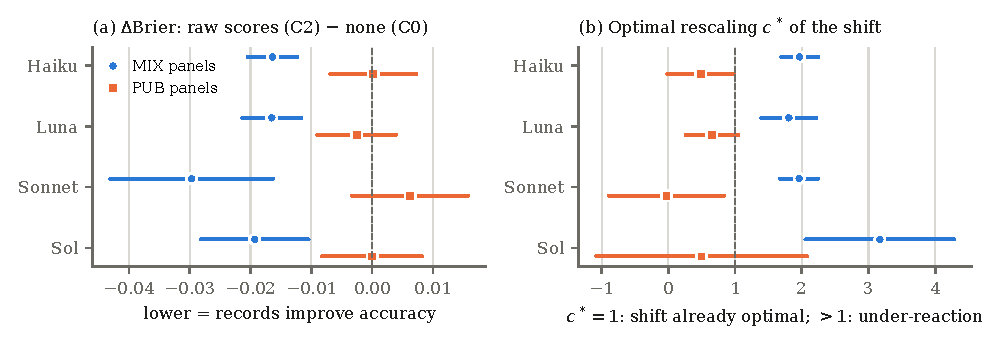
\includegraphics[width=\linewidth]{figures/fig_e1_cstar.pdf}
\caption{(a) Showing a raw mean Brier per forecaster lowers the LLM's Brier score on MIX panels for every model, and has
no measurable effect on PUB panels. (b) The optimal rescaling of each model's record-induced shift is about 2 or more in MIX
(under-reaction) and below 1 in PUB, where the shift adds no demonstrable accuracy. Primary sample; 95\% CIs (two-way
cluster-robust). Haiku and Luna: 486 panels over three draws; Sonnet and Sol: 108 draw-0 panels, a sample more favourable to experts. Do not compare magnitudes across the two pairs.}
\label{fig:e1}
\end{figure}

\begin{table}[t]
\centering\small
\caption{RQ1--RQ2 detail. Oracle fraction (C2, MIX, primary); E1 in PUB;
held-out Brier change from rescaling by a cross-fitted $\cstar$ (negative = rescaling helps); and the direct MIX$-$PUB
difference in $\cstar$ with question-bootstrap CI. Held-out rescaled forecasts are clipped to [0.001, 0.999].}
\label{tab:rq12}
\setlength{\tabcolsep}{4pt}
\resizebox{\linewidth}{!}{\begin{tabular}{@{}llllll@{}}
\toprule
Model & Oracle frac. & E1 PUB & Held-out gain MIX & Held-out gain PUB & $\cstar_{\text{MIX}}-\cstar_{\text{PUB}}$ \\
\midrule
Haiku & 0.62 [0.47, 0.78] & 0.000 [\ensuremath{-}0.007, 0.007] & \ensuremath{-}0.0059 [\ensuremath{-}0.0095, \ensuremath{-}0.0022] & \ensuremath{-}0.0004 [\ensuremath{-}0.0035, 0.0027] & 1.48 [0.99, 2.02] \\
Luna & 0.63 [0.49, 0.76] & \ensuremath{-}0.003 [\ensuremath{-}0.009, 0.004] & \ensuremath{-}0.0049 [\ensuremath{-}0.0085, \ensuremath{-}0.0011] & \ensuremath{-}0.0003 [\ensuremath{-}0.0024, 0.0019] & 1.15 [0.65, 1.67] \\
Sonnet & 0.78 [0.53, 1.02] & 0.006 [\ensuremath{-}0.003, 0.016] & \ensuremath{-}0.0123 [\ensuremath{-}0.0187, \ensuremath{-}0.0065] & \ensuremath{-}0.0035 [\ensuremath{-}0.0173, 0.0121] & 1.99 [0.90, 3.38] \\
Sol & 0.51 [0.33, 0.68] & 0.000 [\ensuremath{-}0.008, 0.008] & \ensuremath{-}0.0233 [\ensuremath{-}0.0341, \ensuremath{-}0.0125] & 0.0028 [\ensuremath{-}0.0013, 0.0076] & 2.67 [0.70, 4.58] \\
\bottomrule

\end{tabular}}
\end{table}

\subsection{RQ1: records help when experts are present, but less than a simple rule}
On MIX panels, raw scores (C2) lower the Brier score for all four models (Table~\ref{tab:conf}, Fig.~\ref{fig:e1}a),
so the pre-registered ``all models'' criterion is met. On the common sample, the improvement is \eOneCommonHaiku{}
(Haiku), \eOneCommonLuna{} (Luna), \eOneCommonSonnet{} (Sonnet) and \eOneCommonSol{} (Sol). This sample is the most
favourable to experts of the three draws, so the tiers' primary numbers should not be compared. The models capture
\oracleFracSol--\oracleFracSonnet{} of the gain available from knowing who the superforecasters are
(Table~\ref{tab:rq12}). On PUB panels, $\Delta$Brier is indistinguishable from zero for every model.
Format matters: itemised records (C1) help Luna and Sol about as much as C2, but not Haiku (oracle fraction
\oracleFracConeHaiku{}) and barely Sonnet (\oracleFracConeSonnet{}). Peer-relative scores (C3) help less than raw scores for
every model (\oracleFracCthreeHaiku--\oracleFracCthreeLuna).

The key qualification is in Fig.~\ref{fig:base} and Table~\ref{tab:base}. With records, every LLM beats the equal mean,
the median and an untuned inverse-Brier rule. \emph{None} beats the cross-validated performance-weighted mean $W$. Luna
and Sol are significantly worse than it on their own panels, and Haiku is too on the common sample (\haikuCommonW,
SE \haikuCommonWse). The superforecaster-only oracle beats three of the four models. In PUB
panels, no predictor beats the equal mean, including $W$ (Brier \pubBrierWHaiku{} against \pubBrierMeanHaiku{}), and $W$
is nominally worse than every LLM (significantly for Sonnet: \pubWSonnet{} [\pubWLoSonnet, \pubWHiSonnet]).

\begin{figure}[t]
\centering
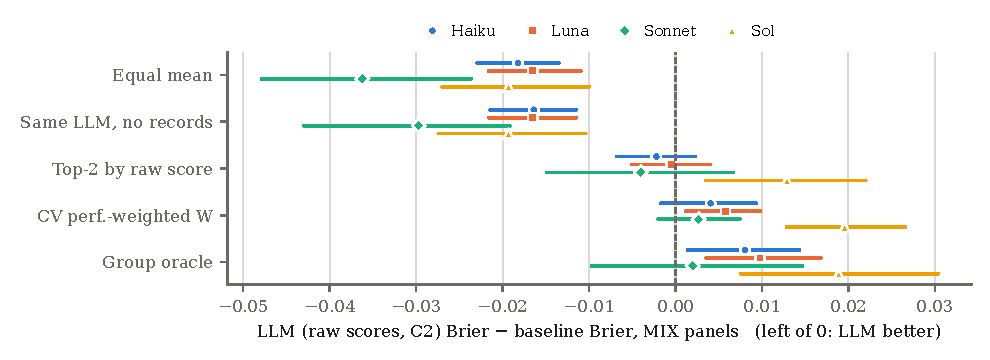
\includegraphics[width=\linewidth]{figures/fig_baselines.pdf}
\caption{Paired Brier differences (LLM with raw scores minus baseline) on MIX panels, with question-cluster
bootstrap 95\% CIs. LLMs beat the mean and their own no-record answers, but not a cross-validated
performance-weighted mean $W$ or the expert oracle. Haiku and Luna: 486 panels over three draws; Sonnet and Sol: 108 draw-0 panels, a sample more favourable to experts. Do not compare magnitudes across the two pairs.}
\label{fig:base}
\end{figure}

\begin{table}[t]
\centering\small
\caption{LLM (C2) Brier minus baseline Brier, MIX panels. Negative means the LLM is better. \textbf{Bold}: the
question-cluster bootstrap 95\% CI excludes 0. Haiku and Luna: 486 panels over three draws; Sonnet and Sol: 108 draw-0 panels, a sample more favourable to experts. Do not compare magnitudes across the two pairs.}
\label{tab:base}
\begin{tabular}{@{}lrrrr@{}}
\toprule
LLM C2 minus\ldots & Haiku & Luna & Sonnet & Sol \\
\midrule
Equal mean & \textbf{\ensuremath{-}0.018} & \textbf{\ensuremath{-}0.017} & \textbf{\ensuremath{-}0.036} & \textbf{\ensuremath{-}0.019} \\
Median & \textbf{\ensuremath{-}0.014} & \textbf{\ensuremath{-}0.012} & \textbf{\ensuremath{-}0.030} & \textbf{\ensuremath{-}0.013} \\
Untuned inverse-Brier & \textbf{\ensuremath{-}0.011} & \textbf{\ensuremath{-}0.009} & \textbf{\ensuremath{-}0.027} & \textbf{\ensuremath{-}0.010} \\
Same LLM, no records (C0) & \textbf{\ensuremath{-}0.016} & \textbf{\ensuremath{-}0.017} & \textbf{\ensuremath{-}0.030} & \textbf{\ensuremath{-}0.019} \\
Top-2 by raw score & \ensuremath{-}0.002 & 0.000 & \ensuremath{-}0.004 & \textbf{\ensuremath{+}0.013} \\
CV perf.-weighted $W$ & \ensuremath{+}0.004 & \textbf{\ensuremath{+}0.006} & \ensuremath{+}0.003 & \textbf{\ensuremath{+}0.020} \\
Group oracle (super mean) & \textbf{\ensuremath{+}0.008} & \textbf{\ensuremath{+}0.010} & \ensuremath{+}0.002 & \textbf{\ensuremath{+}0.019} \\
\bottomrule

\end{tabular}
\end{table}

\subsection{RQ2: under-reaction in MIX, but a regime-blind policy}\label{sec:rq2}
In MIX, $\cstar$ is between \estLunaMIXcStarC{} and \estSolMIXcStarC{}, and every CI excludes 1
(Table~\ref{tab:conf}): each model would have done better by moving two to three times as far in the direction the records
moved it. This holds out of sample. When $\cstar$ is fitted on other questions (10 folds), rescaling improves held-out
Brier for every model (Table~\ref{tab:rq12}). It is also robust to dropping the pilot questions, to a question
jackknife, and to dropping high-leverage questions. With swapped records $\cstar$ falls to zero or below
(\swapMin{} to \swapMax; clearly negative for Haiku, \swapHaiku{}, SE \swapSeHaiku, and Luna, \swapLuna{}, SE
\swapSeLuna), so the useful shift comes from the records and is not generic extremising.

Three qualifications narrow this finding. \emph{(i)} It is the same fact as E1 seen from a different angle: under
quadratic loss, capturing a little over half of the oracle gain implies $\cstar\approx2$. \emph{(ii)} The policy is
\emph{regime-blind}. Each model's slope on the displayed-score differences is similar in MIX and PUB (Haiku
\slopeHaikuMix{} vs \slopeHaikuPub{}; Luna \slopeLunaMix{} vs \slopeLunaPub{}; Sonnet \slopeSonnetMix{} vs
\slopeSonnetPub{}; Sol \slopeSolMix{} vs \slopeSolPub{}). The prompt does not say whether experts are present, so
``under-reaction'' means less than an aggregator that knows the panel contains experts, not a failure to read the
scores. \emph{(iii)} ``Two to three times'' is an in-sample magnitude. Even $W$ has an outcome-optimal scale above 1
(\betaStarEff{} and \betaStarStrong{} in the two samples), and the ex-ante statement is that the models move
\betaBaseMin--\betaBaseMax{} as far as $W$.

In PUB, $\cstar<1$ for every model. The frozen design labelled this over-reaction; we do \emph{not} read it that way,
for two reasons found after the run. Only Sonnet passes Holm, and only under the frozen SE convention (Holm
$p=\sonnetPubHolmFrozen$); it fails under two alternative conventions (\sonnetPubHolmExact{} and, with
question-clustered SEs, \sonnetPubHolmCons). Moreover, $\cstar$ is a through-origin ratio attenuated by sampling noise
in $L_{C2}$: with no record effect and equal noise in both calls, its expected value is $0.5$, not 1. Noise-corrected
PUB values are \noiseCorrPubHaikuA--\noiseCorrPubHaikuB{} (Haiku) and \noiseCorrPubLunaA--\noiseCorrPubLunaB{} (Luna),
and cross-fitted rescaling gives no held-out gain in PUB. What is supported is that in PUB, record-induced shifts add no
demonstrable accuracy. The MIX$-$PUB difference in $\cstar$ is directly supported for every model (Table~\ref{tab:rq12}).


\subsection{RQ3: record farming}\label{sec:rq3}
\textbf{RQ3a (data level, confirmatory).} Over \inflN{} attacker--target pairs, replacing a uniform record with 8
confident items improves the displayed raw mean Brier by \inflRawAbs{} [\inflRawLo, \inflRawHi]. Peer-relative
(\inflPeer{} [\inflPeerLo, \inflPeerHi]) and fixed-effect difficulty-adjusted (\inflFe{} [\inflFeLo, \inflFeHi]) scores
show no inflation. The effect is heterogeneous. Across skill terciles, raw inflation is \inflTercA{}, \inflTercB{} and
\inflTercC{}: for the weakest forecasters, ``easy'' items are not easy, and farming backfires. A normative check
qualifies the threat. Averaged over \normSeedsN{} record draws, a farmed raw score predicts the attacker's target accuracy
slightly \emph{better} than a uniform one (correlation difference \normSeedsMean{}, range \normSeedsMin{} to
\normSeedsMax{}). In these data, a rational aggregator would therefore apply little or no discount.

\textbf{RQ3b (LLM discount): not identified.} The score-matched control often displays exactly the same C2 score as the
farmed record, which would have made the prompts byte-identical and replayed a cached answer. To prevent this, we
appended a line ``\texttt{Cache nonce: control}'' to every control prompt. This made the prompt text depend on the arm.
In \nonceHaikuN{} PUB panels, the C2 control and farmed prompts differ \emph{only} by this line, which gives a natural
experiment: Haiku's answers shift toward the mean (Appendix Table~\ref{tab:nonce}), its reasoning tokens per call fall
from \nonceTokFarm{} to \nonceTokCtl{} in these pairs (\nonceTokFarmAll{} to \nonceTokCtlAll{} over all 486 panels), and the implied contribution to $D$ is \nonceHaikuD{}, matching its failed C2 placebo
(\placeboHaikuDtwo{}). Effects compatible with the nonce also appear for Luna (C3) and Sonnet (C2), and for no model is the
line shown to be inert. The E3b column of Table~\ref{tab:conf} is therefore reported only for completeness. Even
without the nonce, the test would be uninformative. No discount is warranted (RQ3a), so $D\approx0$ is also the rational
response. The minimum detectable effect at 80\% power is \mdeMin--\mdeMax, above any plausible warranted discount. And C1
records show category codes, so farmed and control records also differ in base-rate information. No estimand other than
those using the control or retest arms is affected (Appendix~\ref{app:nonce}).

\subsection{Exploratory analyses (post hoc)}\label{sec:expl}
These analyses were not in the frozen design and have no multiplicity control.
\emph{(a) A regime-blind $W$.} The frozen $W$ is tuned separately for MIX and PUB. We re-tuned the same rule on the
Phase~3 panels with the frozen folds, once per panel type and once pooled over both (assuming a 50/50 mix). Pooling
raises its MIX Brier from \typedWBrier{} to \pooledWBrier. Against the pooled rule in MIX, Luna and Sol remain worse
(\pooledWLuna{} [\pooledWLoLuna, \pooledWHiLuna]; \pooledWSol{} [\pooledWLoSol, \pooledWHiSol]); Haiku is borderline
(\pooledWHaiku{} [\pooledWLoHaiku, \pooledWHiHaiku]) and not robust to a tuning variant that masks held-out questions
from training records (\pooledWMaskedHaiku); Sonnet is nominally better (\pooledWSonnet{} [\pooledWLoSonnet,
\pooledWHiSonnet]). Over MIX and PUB together, Haiku (\pooledWAllHaiku{} [\pooledWAllLoHaiku, \pooledWAllHiHaiku]) and
Luna (\pooledWAllLuna{} [\pooledWAllLoLuna, \pooledWAllHiLuna]) are indistinguishable from the pooled rule, Sol is
nominally worse (\pooledWAllSol{} [\pooledWAllLoSol, \pooledWAllHiSol]) and Sonnet is better (\pooledWAllSonnet{}
[\pooledWAllLoSonnet, \pooledWAllHiSonnet]). Part of $W$'s MIX advantage is therefore knowledge of the regime.
\emph{(b) Stated weights.} The weighted mean implied by each model's stated weights (renormalised) is close to its
reported probability (mean absolute gap at most \pwGapMax) and scores no better (MIX: \pwMinusLlmMin{} to
\pwMinusLlmMax, all CIs include 0). The stated weights imply moving \statedShiftMin--\statedShiftMax{} of the way from
the equal mean to the superforecasters' mean, against \revealedShareMin--\revealedShareMax{} for the answers: the
under-reaction is already in the weights, and asking for weights is not a better recipe.

\section{Discussion and conclusion}
\textbf{What this means for trust infrastructure.} (1) Reliability metadata is useful to an AI aggregator \emph{when
there is real skill dispersion to find}. When there is not, it does not help, and a well-calibrated aggregator should
largely ignore it. (2) Current LLMs read raw scores sensibly but conservatively, and they apply roughly the same policy
whether or not the panel contains experts. In MIX, a transparent cross-validated weighting rule was at least as good as
every model. In PUB no rule beat the plain mean, and the same weighting rule was nominally worse than every LLM
(significantly so for Sonnet). A statistical aggregate is therefore a strong default only when the right rule for the
regime is known. Showing that aggregate to the model, or to the human, is a natural design to test; we did not test
it. (3) Selective-question farming inflates raw mean Brier, and peer-relative or difficulty-adjusted scores neutralise
it. The threat is modest here: farmed scores were no less predictive of target accuracy than uniform ones. Score designers can obtain this
robustness at little cost, although LLMs used peer-relative scores less effectively than raw ones (C3 oracle fraction
\oracleFracCthreeHaiku--\oracleFracCthreeLuna). This tension is worth resolving in score presentation.

\subsection*{Limitations}
\emph{Scope:} one ForecastBench round, 162 questions, four models. \emph{Records} are cross-sectional (same round,
not chronological), though they never contain the target. \emph{MIX framing} makes the task ``find the two
superforecasters'', and the models are not told that experts may be present. \emph{Strong tier:} 108 questions at
draw 0; cross-model contrasts are confounded with reasoning (Sonnet emits no reasoning tokens). \emph{Routing:}
OpenRouter served the Anthropic models from three upstream providers, with balanced shares across conditions.
\emph{Standard errors:} the frozen two-way SE lacks a small-sample correction; one PUB cell depends on the SE
convention and is not interpreted. \emph{In-sample magnitudes:} rescaling by $\cstar$ would push 14--18\% of MIX
forecasts outside $[0,1]$. \emph{Farming:} E3b is not identified, and the fixed-effect abilities in E3a were fitted on
data that include the target questions. \emph{Multiplicity:} the common-sample Holm correction divides by 4 for a
3-test family (conservative); post hoc analyses have no multiplicity control. \emph{Dual use:} the paper describes how
to pad a record, alongside the defence (peer-relative scoring).

\subsection*{Future work} A farming test needs an arm in which a discount \emph{is} warranted, for example records farmed
from a skill-uncorrelated pool, with power computed against that warranted effect. Cache-busting must go into request
settings (for example a seed), never into prompt text. Next steps: regime-aware prompts, showing the statistical aggregate
alongside the records, and chronologically built records from several rounds.

\section*{AI use and process disclosure}
This project was planned, implemented and analysed by AI agents under human direction. An Opus-class model led design
and analysis; a Codex model implemented the engineering; a separate Claude model, as independent reviewer, audited the
design and the results and reproduced every confirmatory number (to within $10^{-15}$). The human author set the
question, budget and constraints, and approved each paid phase. API spend was \$12.52 of a \$20 budget. No result was
fitted on held-out outcomes, no analysis was rerun to change a significance call, and all deviations from the frozen
design (including the nonce flaw) are logged in the repository.

\bibliographystyle{plainnat}
\bibliography{refs}

\appendix
\section{Reproducibility and claims ledger}\label{app:repro}
All 19,876 raw responses are committed (gzipped) with frozen panels, manifests and configs. The frozen analysis
(\texttt{scripts/analyze\_phase3.py}) generates every confirmatory estimand. Independent recomputations by the lead
(\texttt{results/lead\_recompute/}) and the reviewer (\texttt{results/review\_phase3/}) agree with it: the reviewer
reproduced 164 frozen estimand rows, including every confirmatory estimate, SE and $p$-value, to within
$8.9\times10^{-16}$, and the lead reproduced the 48 headline E1 and $\cstar$ estimates. Every number in this paper is a \LaTeX{} macro generated by
\texttt{paper/make\_numbers.py}. \texttt{paper/generated/claims\_ledger.csv} maps each macro to its source file and row.
Design constants (sample sizes, $k$, thresholds) and process figures (cost) are typed and are listed in
\texttt{paper/CLAIMS.md}.

\section{Nonce audit}\label{app:nonce}
\begin{table}[h]
\centering\small
\caption{Identical-text pairs: PUB panels where the control and farmed prompts differ only by the nonce line. Mean
(control $-$ farmed) probability, implied contribution to $D$, and change in reasoning tokens per call.
Question-cluster bootstrap 95\% CIs; \textbf{bold} excludes 0.}
\label{tab:nonce}
\resizebox{\linewidth}{!}{\begin{tabular}{@{}llrllr@{}}
\toprule
Model & Arm & $n$ & Mean shift & $D$ contribution & $\Delta$ reasoning tok. \\
\midrule
Haiku & C2 & 373 & \textbf{\ensuremath{-}0.0124 [\ensuremath{-}0.0189, \ensuremath{-}0.0065]} & \textbf{\ensuremath{-}0.029 [\ensuremath{-}0.053, \ensuremath{-}0.006]} & \ensuremath{-}197 \\
Haiku & C3 & 417 & \ensuremath{-}0.0005 [\ensuremath{-}0.0035, 0.0026] & \ensuremath{-}0.006 [\ensuremath{-}0.018, 0.007] & \ensuremath{-}18 \\
Luna & C2 & 373 & \ensuremath{+}0.0011 [\ensuremath{-}0.0027, 0.0049] & \ensuremath{-}0.002 [\ensuremath{-}0.015, 0.012] & \ensuremath{+}5 \\
Luna & C3 & 417 & \textbf{\ensuremath{-}0.0032 [\ensuremath{-}0.0060, \ensuremath{-}0.0004]} & \textbf{\ensuremath{-}0.018 [\ensuremath{-}0.029, \ensuremath{-}0.008]} & \ensuremath{+}2 \\
Sonnet & C2 & 90 & \textbf{\ensuremath{+}0.0038 [0.0011, 0.0070]} & \ensuremath{+}0.004 [\ensuremath{-}0.007, 0.015] & 0 \\
Sol & C2 & 90 & \ensuremath{+}0.0005 [\ensuremath{-}0.0017, 0.0027] & \ensuremath{-}0.005 [\ensuremath{-}0.013, 0.003] & 0 \\
\bottomrule

\end{tabular}}
\end{table}
Unaffected estimands: E1, the oracle fraction, $\cstar$ (including cross-fitted values and the MIX$-$PUB contrast),
the $W$-relative scale $\beta$, swap checks, baselines, the probe, and E3a. Affected: $D_{C1}$, $D_{C2}$ and $D_{C3}$ (not interpretable),
and the retest SD (an upper bound on sampling noise).

\section{Additional checks}\label{app:extra}
\begin{itemize}
\item \textbf{Probe (question text, no forecasts):} Brier \probeHaiku{} (Haiku), \probeLuna{} (Luna), \probeSonnet{}
  (Sonnet), \probeSol{} (Sol), against crowd \probeCrowdLo--\probeCrowdHi. Pretraining knowledge is plausible, so the
  main prompts rely on anonymisation.
\item \textbf{Robustness:} E1 MIX and $\cstar$ MIX remain Holm-significant for every model when the 16 pilot questions
  are excluded, on the common sample, and under four SE conventions.
\item \textbf{Swap check:} with C2 records, 95--100\% of swaps move the aggregate in the expected direction.
\end{itemize}

\end{document}
